\chapter{Beschreibung des 5G-AKA Protokolls}
\label{chap:2}

Das 5G-AKA-Protokoll ist eines von mehreren Protokollen des 5G-Standards.
Vor Allem das EAP-AKA-Protokoll und das 5G-AKA-Protokoll sind f\"ur den sicheren Austausch eines Schl\"ussels zust\"andig. 
Bei beiden Protokollen ist der erste Teil der Gleiche bis bei dem Provider eines der Protokolle ausgew\"ahlt wird. %3GPP TS 33.501 V15.34.1 Page 40
Bei beiden Protokollen ist auch der Authentifizierungsvorgang sehr \"ahnlich, wobei jedoch der das 5G-AKA-Protokoll das EAP-AKA-Protokoll darum erweitert, dass es dem Provider, ''home network'' genannt, eine erfolgreiche Authentifizierung nachweist. %3GPP TS 33.501 V15.34.1 Page 43

Das 5G-AKA-Protokoll wird gr\"o{\ss}tenteils in der Spezifikation TS 33.501 des 3GPP beschrieben. %3GPP TS 33.501 V15.34.1
Dabei wird die zurzeit neueste Version V15.34.1 herangezogen.

\section{Ziele}

TODO

\section{Das Protokoll}

\subsection{Entities}

In dem Protokoll werden vier grundlegende Entit\"aten beschrieben.
Diese sind das \gls{ue}, die \gls{seaf}, die \gls{ausf} und das \gls{udm}.

\glsreset{ue}
\subsubsection{\gls{ue}}

Das \gls{ue} befindet sich auf dem Smartphone des Nutzers.
Es l\"asst sich in das \gls{me} und das \gls{usim} unterteilen.
In dem \gls{usim} werden f\"ur die Authentifizierung ben\"otigte Schl\"ussel und Benutzerkennungen gespeichert, die f\"ur die eindeutige Identifizierung und Authentifizierung des \gls{ue} ben\"otigt werden. %3GPP TS 33.501 V15.34.1 Page 24
In dem \gls{me} werden die Schl\"ussel, die f\"ur die Kommunikation nach dem 5G-AKA-Protokoll ben\"otigt werden berechnet.

\glsreset{seaf}
\subsubsection{\gls{seaf}}

Die \gls{seaf} ist Teil des mit dem \gls{ue} kommunizierenden Netzwerks, auch \textit{''Serving Network''‚} genannt.
Sie kommuniziert mit dem \gls{ue} und mit dem korrekten Provider des Benutzers.
Nach erfolgreicher Authentifizierung haben das \gls{ue} und die \gls{seaf} beide einen gemeinsamen Schl\"ussel.%3GPP TS 33.501 V15.34.1 Page 37

\glsreset{ausf}
\subsubsection{\gls{ausf}}

Die \gls{ausf} ist Teil des Providers, bei dem sich der Benutzer die hier verwendete SIM-Karte gekauft hat, auch \textit{''Home Environment''} genannt.
Sie kommuniziert mit der \gls{seaf} und validiert die Antwort des \gls{ue} f\"ur die \gls{seaf}.

\glsreset{udm}
\subsubsection{\gls{udm}}

Das \gls{udm} ist, wie auch die \gls{ausf} Teil des \textit{''Home Environment''}.
Grunds\"atzlich funktioniert es jedoch nicht ohne die \gls{arpf} und die \gls{sidf}.

Das \gls{udm} und die \gls{arpf} generieren Authentifizierungsvektoren aus den Schl\"usseln, die sie mit dem \gls{usim} teilen.
Die \gls{sidf} gerechnet die Benutzerkennung (\glsunset{supi}\gls{supi}) f\"ur den \gls{udm} und die \gls{arpf} aus einer verschl\"usselten Benutzerkennung (\glsunset{suci}\gls{suci}), die sie von dem \gls{ausf} erh\"alt.


\subsection{Wichtige Definitionen}
\glsunset{5g-guti}
\glsunset{5g-he-av}
\glsunset{5g-se-av}
\glsunset{ak}
\glsunset{amf}
\glsunset{autn}
\glsunset{ck}
\glsunset{f12345}
\glsunset{hres*}
\glsunset{hxres*}
\glsunset{ik}
\glsunset{imsi}
\glsunset{k}
\glsunset{k-ausf}
\glsunset{k-seaf}
\glsunset{kdf}
\glsunset{mac}
\glsunset{mcc}
\glsunset{mnc}
\glsunset{rand}
\glsunset{res}
\glsunset{res*}
\glsunset{sidf}
\glsunset{sn-name}
\glsunset{sqn}
\glsunset{suci}
\glsunset{supi}
\glsunset{supi-type}
\glsunset{xmac}
\glsunset{xres}
\glsunset{xres*}

\glsreset{5g-guti}
\subsubsection{\gls{5g-guti}}
Der \gls{5g-guti} kann wie auch der \gls{suci}, f\"ur die Initiierung der Authentifizierung verwendet werden.
Er besteht aus zwei Teilen mit denen man das \gls{amf}, welches den \gls{5g-guti} erstellt hat, und das \gls{ue}, welches dem \gls{5g-guti} zugeordnet wurde, eindeutig identifizieren kann. %3GPP TS 23.003 V15.7.0 Page 35
Diese Teile sind der \gls{guami} und der \gls{5g-tmsi}.

\gls{5g-guti} = \gls{guami} || \gls{5g-tmsi}

\gls{guami} = \gls{mcc} || \gls{mnc} || AMF Identifier

AMF Identifier = AMF Region Id || AMF Set Id || AMF Pointer

Der \gls{5g-tmsi} hat eine L\"ange von 32 Bits, die AMF Region Id hat eine L\"ange von 8 Bits, die AMF Set Id hat eine L\"ange von 10 Bits und der AMF Pointer hat eine L\"ange von 6 Bits. %3GPP TS 23.003 V15.7.0 Page 36

\glsreset{5g-he-av}
\subsubsection{\gls{5g-he-av}}
Der \gls{5g-he-av} wird von dem \gls{udm} erstellt und an die \gls{ausf} geschickt.

Er beinhaltet \gls{rand}, \gls{autn}, \gls{xres*} und \gls{k-ausf}. %3GPP TS 33.501 V15.34.1 Page 44

\glsreset{5g-se-av}
\subsubsection{\gls{5g-se-av}}
Der \gls{5g-se-av} wird von der \gls{ausf} erstellt und an die \gls{seaf} geschickt.

Er beinhaltet \gls{rand}, \gls{autn} und \gls{hxres*}. %3GPP TS 33.501 V15.34.1 Page 44

\glsreset{ak}
\subsubsection{\gls{ak}}
Der \gls{ak} hat eine L\"ange von 48 Bits und wird zum verschl\"usseln der \gls{sqn} verwendet. %3GPP TS 33.102 V15.1.0 Page 32
L\"asst die \gls{sqn} keine R\"uckschl\"usse auf die Identit\"at oder Position der Nutzers zu so kann der \gls{ak} auch auf 0 gesetzt werden. %3GPP TS 33.102 V15.1.0 Page 25

Der \gls{ak} wird mit der \textit{''Key generating function''} f5 berechnet. Diese Funktion bekommt \gls{rand} als Eingabe und ist von \gls{k} abh\"angig. %3GPP TS 33.102 V15.1.0 Page 26

\glsreset{amf}
\subsubsection{\gls{amf}}
Das \gls{amf} ist eine 16 Bit lange Zahl. %3GPP TS 33.102 V15.1.0 Page 32
Die 16 Bits des \gls{amf} sind von ''0'' bis ''15'' durchnummeriert. %3GPP TS 33.102 V15.1.0 Page 79
0 steht hier f\"ur das \textit{''most significant bit''} und 15 steht f\"ur das \textit{''least significant bit''}.

\begin{itemize}
\item Bit ''0'', auch \textit{''separation bit''} genannt, wird f\"ur das \gls{eps} verwendet und wird bei der Verwendung des \gls{amf} mei{\ss}t explizit angegeben. \\
\item Bits ''1'' bis ''7'' sind f\"ur eine zuk\"unftige Spezifikation reserviert und sollen auf 0 gesetzt werden. \\
\item Bits ''8'' bis ''15'' k\"onnen f\"ur propriet\"are Zwecke verwendet werden, sind aber nicht explizit festgelegt. 
Sie k\"onnen verwendet werden um providerspezifische Anpassungen festzulegen.
Zum Beispiel k\"onnten mehrere Authentifikations-Algorithmen unterst\"utzt werden, indem die Bits ''8'' bis ''15'' den Algorithmus festlegen oder es k\"onnten die Verifikationsparameter der \gls{sqn} durch die Bits bestimmt werden. %3GPP TS 33.102 V15.1.0 Page 77
\end{itemize}

\glsreset{autn}
\subsubsection{\gls{autn}}
Der \gls{autn} besteht aus den drei Komponenten \gls{sqn}$ \oplus $\gls{ak}, \gls{amf} und \gls{mac}. 
Er ist wie folgt aufgebaut: %3GPP TS 33.102 V15.1.0 Page 25

\gls{autn} = \gls{sqn}$ \oplus $\gls{ak} || \gls{amf} || \gls{mac}

\begin{itemize}
\item Das \gls{amf} wird ben\"otigt um \gls{mac} zu berechen und um providerspezifische Anpassungen vorzunehmen.
\item Der \gls{mac} wird ben\"otigt um ihn mit dem \gls{xmac} zu vergleichen.
\item Die \gls{sqn}$ \oplus $\gls{ak} soll die \gls{sqn} \"ubermitte\"ln.
Sie wird mit dem \gls{ak} verschl\"usselt um die Identit\"at und Position der Benutzers nicht preiszugeben.
Ist \gls{ak} = 0, dann kann davon ausgegangen werden dass die \gls{sqn} alleine weder Identit\"at noch Position des Benutzers preisgibt.
\end{itemize}

\glsreset{ck}
\subsubsection{\gls{ck}}
Der \gls{ck} ist ein 128 Bit langer Schl\"ussel. %3GPP TS 33.102 V15.1.0 Page 32
Er wird von der \textit{''Key generating function''} f3 berechnet.
Diese Funktion ist von \gls{k} abh\"angig und bekommt \gls{rand} als Eingabe. %3GPP TS 33.102 V15.1.0 Page 26

Der \gls{ck} und der \gls{ik} werden ben\"otigt um \gls{k-ausf} zu berechnen.

\glsreset{f12345}
\subsubsection{\gls{f12345}}
Mit diesen Funktionen werden \gls{ak}, \gls{ck}, \gls{ik} \gls{res} bzw. \gls{xres} und \gls{mac} bzw. \gls{xmac} berechnet. %3GPP TS 33.102 V15.1.0 Page 26
\begin{itemize}
\item f1 ist eine \textit{''Message authentication function''}.
Sie berechnet in Abh\"angigkeit von \gls{k} den \gls{mac} bzw. \gls{xmac} und bekommt als Eingabe die Konkatenation von \gls{sqn}, \gls{rand} und \gls{amf} (\gls{sqn} || \gls{rand} || \gls{amf}). \\
\item f2 ist eine, m\"oglicherweise verk\"urzte, \textit{''Message authentication function''}.
Sie berechnet in Abh\"angigkeit von \gls{k} die \gls{res} bzw. \gls{xres} und bekommt \gls{rand} als Eingabe.
\item f3, f4 und f5 sind \textit{''Key generating functions''}.
f3 berechnet \gls{ck}, f4 berechnet \gls{ik} und f5 berechnet \gls{ak}.
Alle drei bekomment \gls{rand} als Eingabe und sind abh\"angig von \gls{k}.
Falls \gls{sqn} keine R\"uckschl\"usse auf die Identit\"at oder Position des Benutzers zul\"asst wird f5 = 0 gesetzt.
\end{itemize}

\glsreset{hres*}
\subsubsection{\gls{hres*}}
\gls{hres*} ist der Hash von \gls{res*}.
Er wird von der \gls{seaf} mit Hilfe des SHA-256-Algorithmus berechnet. %3GPP TS 33.501 V15.34.1 Page 155
Eingabe des SHA-256-Algorithmus ist die Konkatenation von \gls{rand} und \gls{res*} (\gls{rand} || \gls{res*}).

\gls{hres*} setzt sich aus den 128 \textit{''least significant''} Bits von der Ausgabe des SHA-256 zusammen.

\glsreset{hxres*}
\subsubsection{\gls{hxres*}}
\gls{hxres*} ist der Hash von \gls{xres*}.
Er wird von der \gls{ausf} mit Hilfe des SHA-256-Algorithmus berechnet. %3GPP TS 33.501 V15.34.1 Page 155
Eingabe des SHA-256-Algorithmus ist die Konkatenation von \gls{rand} und \gls{xres*} (\gls{rand} || \gls{xres*}).

\gls{hxres*} setzt sich aus den 128 \textit{''least significant''} Bits von der Ausgabe des SHA-256 zusammen.

\glsreset{ik}
\subsubsection{\gls{ik}}
Der \gls{ik} ist ein 128 Bit langer Schl\"ussel. %3GPP TS 33.102 V15.1.0 Page 32
Er wird von der \textit{''Key generating function''} f4 berechnet.
Diese Funktion ist von \gls{k} abh\"angig und bekommt \gls{rand} als Eingabe. %3GPP TS 33.102 V15.1.0 Page 26

Der \gls{ik} wird zusammen mit dem \gls{ck} ben\"otigt um \gls{k-ausf} zu berechnen.

\glsreset{imsi}
\subsubsection{\gls{imsi}}
Die \gls{imsi} ist bis zu 15 Zeichen lang und besteht aus dem \gls{mcc}, dem \gls{mnc} und der \gls{msin}. %3GPP TS 23.003 V15.7.0 Page 26

\gls{imsi} = \gls{mcc} || \gls{mnc} || \gls{msin}

Die \gls{msin} ist bis zu 9 Zeichen lang und identifiziert den Benutzer eindeutig. %3GPP TS 23.003 V15.7.0 Page 26

\glsreset{k}
\subsubsection{\gls{k}}
\gls{k} ist ein Langzeitschl\"ussel mit einer L\"ange von 128 oder 256 Bits. %3GPP TS 33.102 V15.1.0 Page 32
Die tats\"achliche L\"ange ist nicht spezifiziert und wird m\"oglicherweise von Provider festgelegt. %3GPP TS 33.102 V15.1.0 Page 32

\gls{k} soll auf dem \gls{udm}/\gls{arpf} und in einer manipulationssicheren Hardwarekomponente auf dem \gls{ue} gespeichert werden.  %3GPP TS 33.501 V15.34.1 Page 29
Er wird f\"ur die Generierung von \gls{ak}, \gls{ck}, \gls{ik} \gls{res} bzw. \gls{xres} und \gls{mac} bzw. \gls{xmac} ben\"otigt. 

\glsreset{k-ausf}
\subsubsection{\gls{k-ausf}}
\gls{k-ausf} l\"asst sich mit Hilfe der \gls{kdf} berechnen.
Dabei sind folgende Werte Eingabeparameter der \gls{kdf}: %3GPP TS 33.501 V15.34.1 Page 154
\begin{itemize}
\item KEY = Konkatenation von \gls{ck} und \gls{ik} (\gls{ck} || \gls{ik})
\item Fc = 0x6A
\item P0 = \gls{sn-name}
\item P1 = Konkatenation von \gls{sqn} und \gls{ak} (\gls{sqn} || \gls{ak}).
\end{itemize}
Die Ausgabe der \gls{kdf} ist der \gls{k-ausf}.

\gls{k-ausf} wird von der \gls{arpf} und dem \gls{ue} berechnet und wird f\"ur die Berechnung von \gls{k-seaf} ben\"otigt.

\glsreset{k-seaf}
\subsubsection{\gls{k-seaf}}
Der \gls{k-seaf}, auch \textit{''Anchor Key''} genannt ist der Schl\"ussel auf den sich alle Entit\"aten bei erfolgreicher Authentifizierung einigen. %3GPP TS 33.501 V15.34.1 Page 37
Er wird von der \gls{ausf} und dem \gls{ue} berechnet und l\"asst sich mit Hilfe der \gls{kdf} berechnen.
Dabei sind folgende Werte Eingabeparameter der \gls{kdf}: %3GPP TS 33.501 V15.34.1 Page 155
\begin{itemize}
\item KEY = \gls{k-ausf}
\item Fc = 0x6C
\item P0 = \gls{sn-name}
\end{itemize}
Die Ausgabe der \gls{kdf} ist der \gls{k-seaf}.

\glsreset{kdf}
\subsubsection{\gls{kdf}}
Die \gls{kdf} wird f\"ur die Berechnung von \gls{k-ausf}, \gls{k-seaf} und \gls{res*} bzw. \gls{xres*} ben\"otigt.

Die Eingabeparameter der \gls{kdf} sind KEY, Fc, P0, $ \dots $, Pn und optional auch L0, $ \dots $, Ln.

Um den Schl\"ussel zu berechnen muss zuerst der Wert S berechnet werden. %3GPP TS 33.220 V15.4.0 Page 46
S ist von den Eingabeparametern Fc und P1,$ \dots $, Pn abh\"angig.
Er l\"asst sich folgenderma{\ss}en zusammensetzen: 

S = Fc || P0 || L0 || P1 || L1 || $ \dots $ || Pn || Ln 

Die L\"ange von allen P1, $ \dots $, Pn ist durch 8 teilbar und L1, $ \dots $, Ln sind genau 16 Bit gro{\ss} und geben die L\"angen der Parameter P1, $ \dots $, Pn an. 
Das hei{\ss}t, dass Li die Anzahl der Bytes, die mindestens ben\"otigt werden um Pi zu speichern, bin\"ar in 16 Bits kodiert. \\
Zum Beispiel: Ist P0 16 Bit und P1 24 Bit lang, dann hat L0 den Wert 0x02 und L1 den Wert 0x03.

Die Ausgabe der \gls{kdf} ist das Ergebnis folgender Rechnung: \\
Ausgabe = HMAC-SHA-256(KEY, S) \\

\glsreset{mac}
\subsubsection{\gls{mac}}
Der \gls{mac} hat eine L\"ange von 64 Bits und wird, wie auch der \gls{xmac}, mit der \textit{''Message authentication function''} f1 berechnet. %3GPP TS 33.102 V15.1.0 Page 32
Die Funktion f1 ist von \gls{k} abh\"angig und bekommt als Eingabe die Konkatenation von \gls{sqn}, \gls{rand} und \gls{amf} (\gls{sqn} || \gls{rand} || \gls{amf}). %3GPP TS 33.102 V15.1.0 Page 26

Der \gls{mac} wird von der \gls{udm}/\gls{arpf} berechnet und an die \gls{ausf} geschickt, damit er im weiteren Verlauf des Protokolls vom \gls{ue} mit dem \gls{xmac} vergleichen werden kann.

\glsreset{mcc}
\subsubsection{\gls{mcc}}
Der \gls{mcc} ist drei Zeichen lang und identifiziert das Land in dem sich der Provider befindet eindeutig. %3GPP TS 23.003 V15.7.0 Page 26

\glsreset{mnc}
\subsubsection{\gls{mnc}}
Der \gls{mnc} ist zwei oder drei Zeichen lang. %3GPP TS 23.003 V15.7.0 Page 26
Die genaue L\"ange ist vom \gls{mcc} abh\"angig und somit von Land zu Land unterschiedlich.
Der \gls{mnc} und der \gls{mcc} zusammen identifizieren den Provider eindeutig.


\glsreset{rand}
\subsubsection{\gls{rand}}
\gls{rand} ist eine 128 Bit lange zuf\"allige Zahl. %3GPP TS 33.102 V15.1.0 Page 32
Sie wird f\"ur die Generierung von \gls{ak}, \gls{ck}, \gls{ik} \gls{res} bzw. \gls{xres} und \gls{mac} bzw. \gls{xmac} ben\"otigt. 
\gls{rand} soll eine unvorhersehbare Zahl sein, wie genau sie generiert wird ist jedoch nicht beschrieben. %3GPP TS 33.102 V15.1.0 Page 25

Sie wird vom \gls{udm}/\gls{arpf} erzeugt und an das \gls{ue} weitergeleitet. Diese Entit\"aten generieren auch die oben genannten Schl\"ussel \gls{ak}, \gls{ck}, \gls{ik}, usw.

\glsreset{res}
\subsubsection{\gls{res}}
Die \gls{res} hat eine variable L\"ange von bis zu 416 Bytes. %3GPP TS 33.102 V15.1.0 Page 32
Sie wird von dem \gls{ue} mit der \textit{''Message authentication function''} f2 berechnet.
Deise Funktion bekommt \gls{rand} als Eingabe und ist von \gls{k} abh\"angig. %3GPP TS 33.102 V15.1.0 Page 26

Die \gls{res} wird von der \gls{ausf} mit der \gls{xres} verglichen.
Stimmen sie nicht \"uberein so bricht die \gls{ausf} die Authentifizierung ab. %3GPP TS 33.501 V15.34.1 Page 45

\glsreset{res*}
\subsubsection{\gls{res*}}
\gls{res*} l\"asst sich, wie auch \gls{xres*}, mit Hilfe der \gls{kdf} berechnen.
Dabei sind folgende Werte Eingabeparameter der \gls{kdf}: %3GPP TS 33.501 V15.34.1 Page 155
\begin{itemize}
\item KEY = Konkatenation von \gls{ck} und \gls{ik} (\gls{ck} || \gls{ik})
\item Fc = 0x6B
\item P0 = \gls{sn-name}
\item P1 = \gls{rand}
\item P2 = \gls{res}
\end{itemize}

\gls{res*} setzt sich aus den 128 \textit{''least significant''} Bits von der Ausgabe der \gls{kdf} zusammen.
\gls{res*} wird f\"ur die Berechnung von \gls{hres*} ben\"otigt.
Es wird vom \gls{ue} berechnet.

\glsreset{sn-name}
\subsubsection{\gls{sn-name}}
Der \gls{sn-name} wird f\"ur die Berechnung von \gls{res*} bzw. \gls{xres*}, \gls{k-ausf} und \gls{k-seaf} ben\"otigt.
Er hat zwei Zwecke: %3GPP TS 33.501 V15.34.1 Page 39
\begin{itemize}
\item Es bindet den \gls{k-seaf}, auch  \textit{''Anchor Key''}  genannt, an die \gls{seaf}, auch \textit{''Serving Network''} genannt, indem es die SN-Id beinhaltet.
\item Es stellt sicher, dass der \textit{''Anchor Key''} nur f\"ur die Authentifizierung in 5G-Netzwerken verwendbar ist, indem es den Service Code ''5G'' beinhaltet.
\end{itemize}
Der \gls{sn-name} ist wie folgt aufgebaut: %3GPP TS 33.501 V15.34.1 Page 39

Er beginnt mit dem Service code ''5G'' gefolgt von dem Trennzeichen '':'' und der SN-Id.
Die SN-Id ist f\"ur jedes \textit{''Serving Network''} unterschiedlich.

\gls{sn-name} = ''5G'' || '':'' || SN-Id

\glsreset{sqn}
\subsubsection{\gls{sqn}}
\gls{sqn} ist eine Zahl mit einer L\"ange von 48 Bits. %3GPP TS 33.102 V15.1.0 Page 32
Aus ihr wird der \gls{mac} bwz. \gls{xmac} erzeugt. %3GPP TS 33.102 V15.1.0 Page 25

F\"ur die Generierugn der \gls{sqn} muss das \gls{udm}/\gls{arpf} folgende Bedingungen erf\"ullen:\\%3GPP TS 33.102 V15.1.0 Page 25
\begin{enumerate}
\item Der Erzeugungsmechanismus der \gls{sqn} soll eine Re-Synchronisations Prozedur beinhalten.\\
\item Falls die \gls{sqn} R\"uckschl\"usse auf die Identit\"at oder Position des Nutzers zul\"asst, dann soll der \gls{ak} verwendet werden um die \gls{sqn} zu verbergen.\\
\item Der Erzeugungsmechanismus soll gegen den \"Uberlauf der \gls{sqn} (\textit{''Wrap around Protection''}) gesch\"utzt sein, da sonst bereits verwendete Schl\"ussel erneut verwendet werden k\"onnten. 
\end{enumerate}

\glsreset{suci}
\subsubsection{\gls{suci}}
Der \gls{suci} ist die verschl\"usselte Version des \gls{supi}.
Er l\"asst sich mit der \gls{sidf} in den \gls{supi} umwandeln.

Er ist wie folgt aufgebaut: %3GPP TS 23.003 V15.7.0 Page 27

\gls{suci} = \gls{supi-type} || Home Network Identifier || Routing Indicator || Protection Scheme Id || Home Network Public Key Id || Scheme Output

\begin{itemize}
\item Der Home Network Identifier ist von dem \gls{supi-type} abh\"angig.
\begin{itemize}
\item Wenn der \gls{supi-type} den \gls{imsi} angibt, dann entspricht der Home Network Identifier dem \gls{mcc} gefolgt von dem \gls{mnc}. (Home Network Identifier = \gls{mcc} || \gls{mnc})
\item Wenn der \gls{supi-type} den Network Specific Identifier angibt, dann entspricht der Home Network Identifier einer \"ahnichen Form des Network Access Identifiers, wie er beim \gls{supi} verwendet wird. (Home Network Identifier = username@realm)
Er ist genauer im Dokument IETF RFC 7542 spezifiziert. %IETF RFC 7542 Page 10 fort folgend
\end{itemize}
\item Der Routing Indicator besteht aus 1 bis zu 4 Zeichen. %3GPP TS 23.003 V15.7.0 Page 28
Er erlaubt es der \gls{seaf} zusammen mit dem Home Network Identifier eine Verbindung mit der korrekten \gls{ausf} aufzubauen.
Falls kein Routing Indicator konfiguriert ist soll er auf 0 gesetzt werden.
\item Der Protection Scheme Identifier kann Werte von 0 bis 15 annehmen.
Die genaue Definition der einzelnen Algorithmen ist im Annex C des 3GPP TS 33.501 V15.34.1 zu finden. %3GPP TS 33.501 V15.34.1 Page 168
\begin{itemize}
\item Der Wert 0 bedeutet, dass das Null Scheme verwendet wird.
\item Der Wert 1 bedeutet, dass das Profile A verwendet wird.
\item Der Wert 2 bedeutet, dass das Profile B verwendet wird.
\item Die Werte 3 bis 11 sind f\"ur zuk\"unftige Spezifikationen reserviert.
\item Die Werte 12 bis 15 sind f\"ur providerspezifische Algorithmen reserviert.
\end{itemize}
\item Der Home Network Public Key Identifier kann Werte von 0 bis 255 annehmen.
Er wird genutzt den Public Key zu identifizieren, der f\"ur die Verschl\"usselung des \gls{supi} verwendet wird.
\item Der Scheme Output ist die Ausgabe des Verschl\"usselungs-Algorithmus.
Die genaue Definition des Scheme Outputs ist im Annex C des 3GPP TS 33.501 V15.34.1 zu finden. %3GPP TS 33.501 V15.34.1 Page 168
\end{itemize}

\glsreset{supi}
\subsubsection{\gls{supi}}
Der \gls{supi} ist f\"ur jeden Nutzer global eindeutig. 
Er ist wie folgt aufgebaut: %3GPP TS 23.003 V15.7.0 Page 27

\gls{supi} = \gls{supi-type} || Home Network Identifier

Der Identifier ist von dem \gls{supi-type} abh\"angig und kann folgende Werte annehmen:

\begin{itemize}
\item Wenn der \gls{supi-type} den \gls{imsi} angibt, dann entspricht der Home Network Identifier dem \gls{imsi}. (Home Network Identifier = \gls{imsi})
\item Wenn der \gls{supi-type} den Network Specific Identifier angibt, dann entspricht der Home Network Identifier dem Network Access Identifier. (Home Network Identifier = Network Access Identifier)
Der Network Access Identifier hat die Form $ username@realm $. 
Er ist genauer im Dokument IETF RFC 7542 spezifiziert. %IETF RFC 7542 Page 10 fort folgend
\end{itemize}

\glsreset{supi-type}
\subsubsection{\gls{supi-type}}
Der \gls{supi-type} kann Werte von 0 bis 7 annehmen. %3GPP TS 23.003 V15.7.0 Page 27
\begin{itemize}
\item Der Wert 0 bedeutet, dass der Home Network Identifier den \gls{imsi} angibt.
\item Der Wert 1 bedeutet, dass der Home Network Identifier den Network Specific Identifier angibt.
\item Die Werte 2 bis 7 sind f\"ur zuk\"unftige Spezifikation reserviert.
\end{itemize}

\glsreset{xmac}
\subsubsection{\gls{xmac}}
Der \gls{xmac} hat eine L\"ange von 64 Bits und wird wie auch der \gls{mac} mit der Funktion f1 berechnet. %3GPP TS 33.102 V15.1.0 Page 32
Die \textit{''Message authentication function''} f1 ist von \gls{k} abh\"angig und bekommt als Eingabe die Konkatenation von \gls{sqn}, \gls{rand} und \gls{amf} (\gls{sqn} || \gls{rand} || \gls{amf}). %3GPP TS 33.102 V15.1.0 Page 27

Der \gls{xmac} wird von dem \gls{ue} berechnet und mit dem \gls{mac} verglichen. 
Den \gls{mac} hat das \gls{ue} bereits von der \gls{seaf} erhalten.
Stimmen \gls{mac} und \gls{xmac} nicht \"uberein, so ist die Authentifizierung fehlgeschlagen. %3GPP TS 33.102 V15.1.0 Page 27

\glsreset{xres}
\subsubsection{\gls{xres}}
Die \gls{xres} hat eine variable L\"ange von bis zu 416 Bytes. %3GPP TS 33.102 V15.1.0 Page 32
Sie wird, wie auch die \gls{res}, mit der \textit{''Message authentication function''} f2 berechnet. 
Diese Funktion ist von \gls{k} abh\"angig undbekommt \gls{rand} als Eingabe. %3GPP TS 33.102 V15.1.0 Page 26

Die \gls{ausf} vergleicht \gls{res} und \gls{xres} miteinander.
Stimmen sie nicht \"uberein so bricht die \gls{ausf} die Authentifizierung ab. %3GPP TS 33.501 V15.34.1 Page 45

\glsreset{xres*}
\subsubsection{\gls{xres*}}
\gls{xres*} l\"asst sich, wie auch \gls{res*}, mit Hilfe der \gls{kdf} berechnen.
Dabei sind folgende Werte Eingabeparameter der \gls{kdf}: %3GPP TS 33.501 V15.34.1 Page 155
\begin{itemize}
\item KEY = Konkatenation von \gls{ck} und \gls{ik} (\gls{ck} || \gls{ik})
\item Fc = 0x6B
\item P0 = \gls{sn-name}
\item P1 = \gls{rand}
\item P2 = \gls{xres}
\end{itemize}

\gls{xres*} setzt sich aus den 128 \textit{''least significant''} Bits von der Ausgabe der \gls{kdf} zusammen.
\gls{xres*} wird f\"ur die Berechnung von \gls{hxres*} ben\"otigt.
Es wird von der \gls{arpf} berechnet.


\subsection{Weitere Begriffe}

\glsreset{abba}
\subsubsection{\gls{abba}}

\glsreset{auts}
\subsubsection{\gls{auts}}

\glsreset{ng-ksi}
\subsubsection{\gls{ng-ksi}}


\subsection{Authentifikationsprozedur}

Die \cref{fig:protocol_v1} zeigt eine erfolgreiche Authentifizierung.
Nach dem Ende der Prozedur haben sich alle Entit\"aten auf den \textit{''Anchor Key''} \gls{k-seaf} geeinigt.
Dieser wird als Grundlage f\"ur die weitere Kommunikation verwendet.

\begin{figure}[H]
  \centering
  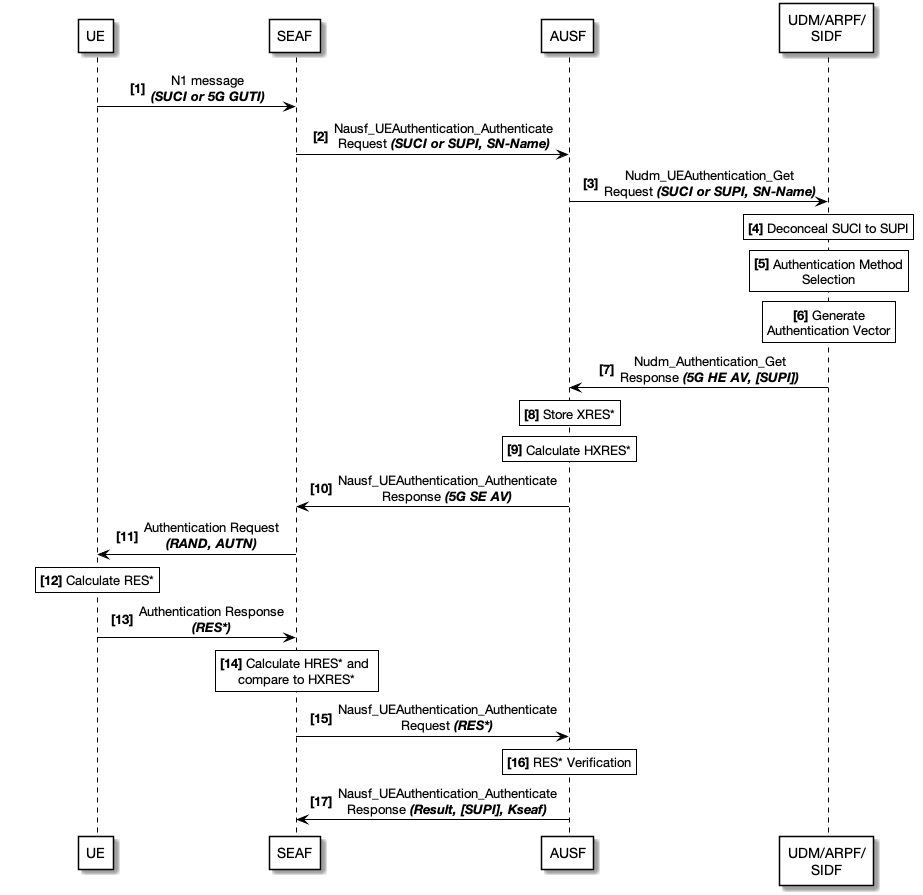
\includegraphics[width=\textwidth]{uml/protocol_v1.png}
  \caption{Erfolgreiche Authentifikation}
  \label{fig:protocol_v1}
\end{figure}

Die einzelnen Nachrichten lassen sich folgenderma{\ss}en beschreiben: %3GPP TS 33.501 V15.34.1 Page 40 und 44

\begin{enumerate}
%1
\item Das \gls{ue} sende in Schritt 1 die \textit{N1 message} an die \gls{seaf} und beginnt damit die Authentifikationsprozedur.
Diese Nachricht beinhaltet entweder den \gls{suci} oder den \gls{5g-guti}.
Sie werden sp\"ater von dem \gls{udm}/\gls{arpf} zur Authentifizierung des \gls{ue} verwendet.

%2
\item Nach dem Empfangen der \textit{N1 message} sendet die \gls{seaf} in Schritt 2 den \textit{Nausf\_UEAuthentication\_Authenticate Request} an die \gls{ausf}.
Falls in der \textit{N1 message} der \gls{5g-guti} enthalten ist und es sich um eine Re-Authentifizierung handelt, dann soll der \gls{supi} an die \gls{ausf} gesendet werden, ansonsten wird der \gls{suci} weitergeleitet.
Zus\"atzlich wird noch der \gls{sn-name} mitgesendet.
Dies ist n\"otig, da das \gls{udm} den \gls{sn-name} f\"ur die Generierung des \gls{5g-he-av} ben\"otigt.

%3
\item Nach dem Empfangen des \textit{Nausf\_UEAuthentication\_Authenticate Request}s checkt die \gls{ausf} ob die \gls{seaf} berechtigt ist den mitgesendeten \gls{sn-name} zu verwenden.
Falls dieser Check erfolgreich war sendet die \gls{ausf} den \textit{Nudm\_UEAuthentication\_Get Request} an das \gls{udm}.
Er enth\"alt den \gls{suci} oder \gls{supi} und den \gls{sn-name}, den die \gls{ausf} aus \textit{Schritt 2} erhalten hat.
Falls der Check nicht erfolgreich war antwortet die \gls{ausf} mit der \textit{Nausf\_UEAuthentication\_Authenticate Response}, die den Text \textit{''serving network not authorized''} enth\"alt.

%4
\item Falls die \gls{ausf} in \textit{Schritt 3} den \gls{suci} an das \gls{udm} gesendet hat, dann wird in diesem Schritt aus dem \gls{suci} der \gls{supi} abgeleitet.
Hierf\"ur wird die \gls{sidf} verwendet.

%5
\item In diesem Schritt wird die Authentifikationsmethode ausgew\"ahlt.
Das \gls{udm} kann zwischen dem EAP-AKA' und dem 5G-AKA Protokoll w\"ahlen.
Da in dieser Ausarbeitung nur auf das 5G-AKA-Protokoll eingegangen wird wird angenommen das hier immer das 5G-AKA-Protokoll als Authentifikationsmethode gew\"ahlt wird.

%6
\item In diesem Schritt wird der \gls{5g-he-av} generiert.
Hierf\"ur wird der \gls{sn-name} und der \gls{supi} ben\"otigt, den das \gls{udm} in \textit{Schritt 3} erhalten oder in \textit{Schritt 4} erzeugt hat.
F\"ur die Generierung soll das \textit{''separation bit''} des \gls{amf} auf ''1'' gesetzt werden.

%7
\item In diesem Schritt sendet das \gls{udm} die \textit{Nudm\_Authentication\_Get Response} an die \gls{ausf}.
Sie beinhaltet den \gls{5g-he-av}, der in \textit{Schritt 6} generiert wurde, und dem Hinweis, dass der \gls{5g-he-av} f\"ur das 5G-AKA-Protokoll bestimmt ist.
Falls das \gls{udm} in \textit{Schritt 3} den \gls{suci} erhalten und in \textit{Schritt 4} den \gls{supi} erzeugt hat, dann wird der \gls{supi} in der \textit{Nudm\_Authentication\_Get Response} mitgeschickt.

%8
\item In Schritt 8 wird die \gls{xres*}, die in dem \gls{5g-he-av} aus \textit{Schritt 7} enthalten ist, und der \gls{suci} oder \gls{supi} zwischengespeichert, da sie in \textit{Schritt 16} f\"ur die Verifikation von \gls{res*} ben\"otigt werden.
Des Weiteren wird auch der \gls{k-ausf}, welcher auch in dem \gls{5g-he-av} enthalten ist, zwischengespeichert.

%9
\item In diesem Schritt wird aus der \gls{xres*} die \gls{hxres*} gerechnet.
Des Weiteren wird der \gls{5g-se-av} f\"ur \textit{Schritt 10} aus dem \gls{5g-he-av} berechnet.
Daf\"ur wird die \gls{xres*} durch die \gls{hxres*} ersetzt und der \gls{k-ausf} entfernt.

%10
\item Nachdem der \gls{5g-se-av} in \textit{Schritt 9} erzeugt wurde wird er in Schritt 10 mit der \textit{Nausf\_UEAuthentication\_Authenticate Response} an die \gls{seaf} gesendet.

%11
\item Nach dem Erhalten der \textit{Nausf\_UEAuthentication\_Authenticate Response} wird die \gls{seaf} in Schritt 11 den \textit{Authentication Request}  an das \gls{ue} schicken.
Er beinhaltet die \gls{rand} und das \gls{autn} den die \gls{seaf} in \textit{Schritt 10} erhalten hat.
Zus\"atzlich wird noch der \gls{ng-ksi} und die \gls{abba}, die nach einer erfolgreiche Authentifizierung ben\"otigt werden, mitgesendet.
Des Weiteren wird die \gls{hxres*}, die in dem \gls{5g-se-av} enthalten ist bei der \gls{seaf} zwischengespeichert, da sie noch f\"ur \textit{Schritt 14} ben\"otigt wird.

%12
\item Nachdem das \gls{ue} den \textit{Authentication Request} von der \gls{seaf} erhalten hat wird in Schritt 12 \"uberpr\"uft ob der \gls{autn} angenommen werden kann.
Ist dies der Fall, dann wird aus der \gls{rand} und dem \gls{autn} die \gls{res*} f\"ur die \textit{Authentication Response} berechnet.
Hierf\"ur wird das \textit{''separation bit''} des \gls{amf} auf ''1'' gesetzt.
Es wird auch der \gls{xmac} berechnet und mit dem \gls{mac}, der in dem \gls{autn} enthalten ist, verglichen.
Stimmen \gls{xmac} und \gls{mac} \"uberein, so wird die Authentifizierung fortgesetzt.
Stimmen sie nicht \"uberein oder kann der \gls{autn} nicht angenommen werden, so wird die Authentifizierung als Fehlgeschlagen angesehen und es wird bei \cref{fig:protocol_mac_failure_v1} weitergemacht.

%13
\item In Schritt 13 wird die \gls{res*}, die in \textit{Schritt 12} berechnet wurde, in der \textit{Authentication Response} vom \gls{ue} an die \gls{seaf} gesendet.

%14
\item Nachdem die \gls{seaf} die \textit{Authentication Response} vom \gls{ue} erhalten hat berechnet sie aus der \gls{res*} die \gls{hres*} und vergleicht sie mit der \gls{hxres*}, die sie in \textit{Schritt 11} zwischengespeichert hat.
Stimmen sie \"uberein so wird bei \textit{Schritt 15} weitergemacht.
Stimmen sie nicht \"uberein, so wird bei dem Abschnitt \textit{''HRES* failure in \gls{seaf}''} in \cref{fig:protocol_res*_verification_failure_v1} weitergemacht.
Wird bis zu einem festgelegten Zeitpunkt keine Antwort vom \gls{ue} erhalten, so wird die Authentifizierung als fehlgeschlagen angesehen und es wird die \gls{ausf} \"uber den Fehlschlag informiert.
Wann dieser Zeitpunkt erreicht ist ist nicht spezifiziert.

%15
\item In Schritt 15 sendet die \gls{seaf} den \textit{Nausf\_UEAuthentication\_Authenticate Request} an die \gls{ausf}.
Er beinhaltet die \gls{res*} den die \gls{seaf} in der \textit{Authentication Response} vom \gls{ue} erhalten hat.

%16
\item Nachdem die \gls{ausf} den \textit{Nausf\_UEAuthentication\_Authenticate Request} erhalten hat vergleicht sie die \gls{res*} mit der \gls{xres*}, die sie in \textit{Schritt 8} zwischengespeichert hat.
Stimmen sie \"uberein so wird bei \textit{Schritt 17} weitergemacht.
Stimmen sie nicht \"uberein, so wird bei dem Abschnitt \textit{''RES* failure in \gls{seaf}''} in \cref{fig:protocol_res*_verification_failure_v1} weitergemacht.
Des Weiteren kann auch \"uberpr\"uft werden ob der Authentication Vector abgelaufen ist.
Dies ist aber nicht zwingend vorgeschrieben.

%17
\item In Schritt 17 sendet die \gls{ausf} die \textit{Nausf\_UEAuthentication\_Authenticate Response} an die \gls{seaf}.
Sie beinhaltet das Ergebnis des Vergleichs von \gls{res*} und \gls{xres*} aus \textit{Schritt 16}.
Stimmen \gls{res*} und \gls{xres*} \"uberein wird auch der \textit{''Anchor Key''} \gls{k-seaf} mitgesendet.
Wenn die \gls{ausf} in \textit{Schritt 7} den \gls{supi} erhalten hat, dann wird im Falle des erfolgreichen Vergleichs von \gls{res*} und \gls{xres*} der \gls{supi} nun auch an die \gls{seaf} weitergeleitet.
\end{enumerate}


\subsection{Fehlgeschlagene Authentifikation}

\subsubsection{Fehlschlag beim Vergleich von \gls{mac} und \gls{xmac}}

\begin{figure}[H]
  \centering
  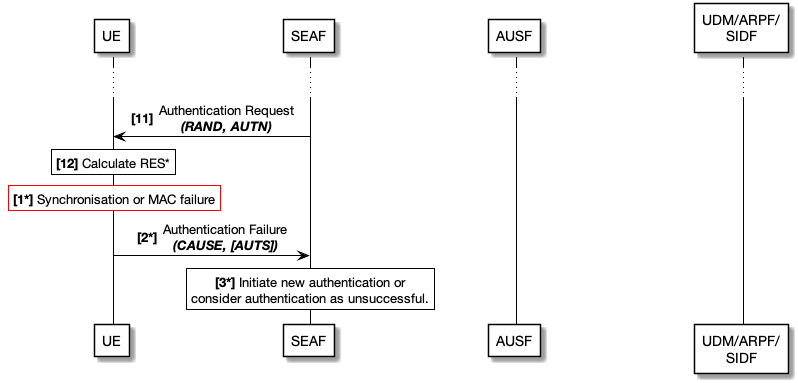
\includegraphics[width=\textwidth]{uml/protocol_mac_failure_v1.png}
  \caption{Fehlschlag beim Vergleich von \gls{mac} und \gls{xmac}}
  \label{fig:protocol_mac_failure_v1}
\end{figure}

\begin{enumerate}
%1*
\item[1*.] In Schritt 1* wird festgestellt, dass der berechnete \gls{xmac} nicht mit dem \gls{mac}, der in Schritt 11 empfangen wurde, \"ubereinstimmt (\textit{''MAC failure''}) oder, dass der \gls{autn} nicht angenommen werden kann (\textit{''Synchronisation failure''}).

%2*
\item[2*.] In Schritt 2* sendet das \gls{ue} die \textit{Authentication Failure} an die \gls{seaf}.
Sie beinhaltet den CAUSE Wert, welcher den Grund f\"ur das Fehlschlagen beschreibt.
Handelt es sich um eine \textit{''Synchronisation failure''} so wird auch der \gls{auts} Parameter mitgesendet.

%3*
\item[3*.] In Schritt 3* wird entschieden ob die Authentifikation gescheitert ist oder ob eine neue Authentifikation initiiert werden soll.
eine neue Authentifikation kann nur initiiert werden wenn es sich bei dem Fehlschlag um eine \textit{''Synchronisation failure''} handelt.
Die genaue Beschreibung der Re-Authentifizierungsprozedur ist im Dokument TS 24.501 zu finden. %3GPP TS 24.501 V16.1.0
\end{enumerate}


\subsubsection{Fehlschlag beim Vergleich von \gls{res*} bzw. \gls{hres*} mit \gls{xres*} bzw. \gls{hxres*}}

\begin{figure}[H]
  \centering
  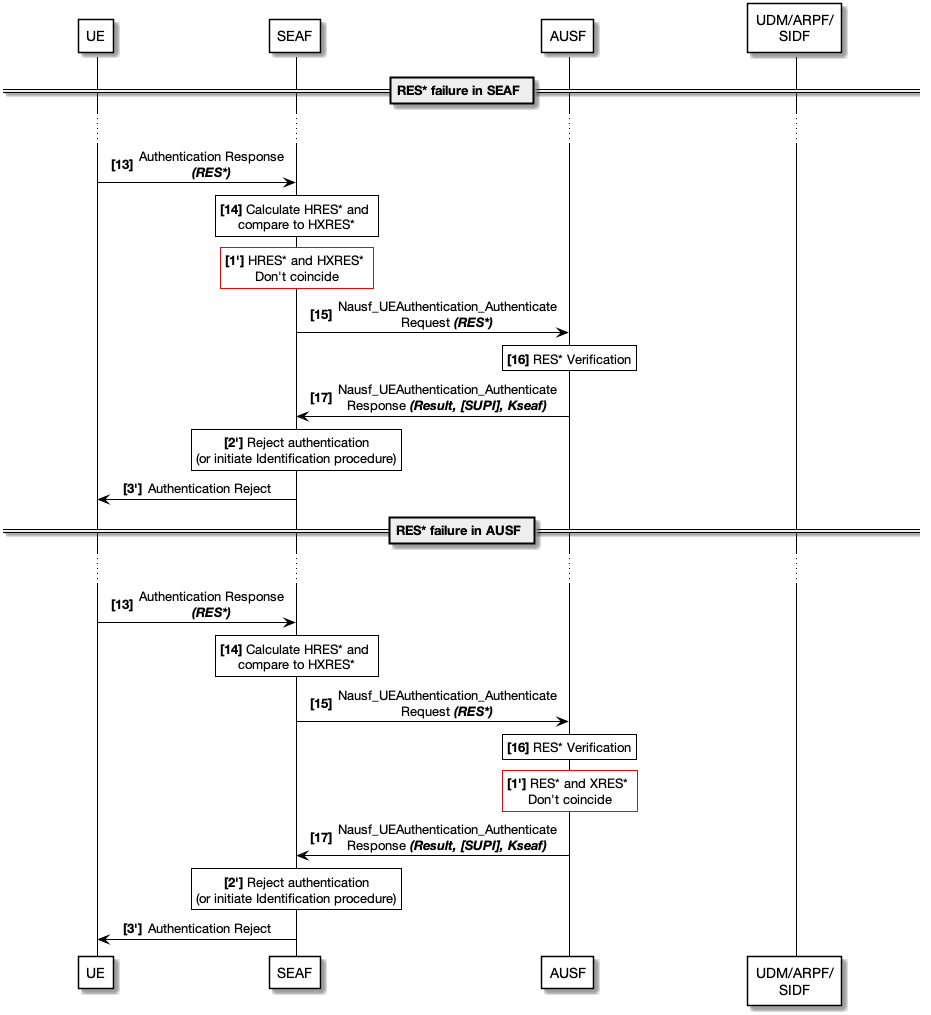
\includegraphics[width=\textwidth]{uml/protocol_res*_verification_failure_v1.png}
  \caption{Fehlschlag beim Vergleich von \gls{res*} bzw. \gls{hres*} mit \gls{xres*} bzw. \gls{hxres*}}
  \label{fig:protocol_res*_verification_failure_v1}
\end{figure}















